\let\negmedspace\undefined
\let\negthickspace\undefined
\documentclass[journal]{IEEEtran}
\usepackage[a5paper, margin=10mm, onecolumn]{geometry}
\usepackage{tfrupee} 
\setlength{\headheight}{1cm} 
\setlength{\headsep}{0mm}     

\usepackage{gvv-book}
\usepackage{gvv}
\usepackage{cite}
\usepackage{amsmath,amssymb,amsfonts,amsthm}
\usepackage{algorithmic}
\usepackage{graphicx}
\usepackage{textcomp}
\usepackage{xcolor}
\usepackage{txfonts}
\usepackage{listings}
\usepackage{enumitem}
\usepackage{mathtools}
\usepackage{gensymb}
%\usepackage{wasysym}
\usepackage{comment}
\usepackage[breaklinks=true]{hyperref}
\usepackage{tkz-euclide} 
\usepackage{listings}
\def\inputGnumericTable{}                                 
\usepackage[latin1]{inputenc}                                
\usepackage{color}                                            
\usepackage{array}                                            
\usepackage{longtable}                                       
\usepackage{calc}                                             
\usepackage{multirow}                                         
\usepackage{hhline}                                           
\usepackage{ifthen}                                           
\usepackage{lscape}
\usepackage{circuitikz}
\tikzstyle{block} = [rectangle, draw, fill=blue!20, 
    text width=4em, text centered, rounded corners, minimum height=3em]
\tikzstyle{sum} = [draw, fill=blue!10, circle, minimum size=1cm, node distance=1.5cm]
\tikzstyle{input} = [coordinate]
\tikzstyle{output} = [coordinate]
\renewcommand{\thefigure}{\theenumi}
\renewcommand{\thetable}{\theenumi}
\setlength{\intextsep}{10pt} % Space between text and floats
\numberwithin{equation}{enumi}
\numberwithin{figure}{enumi}
\renewcommand{\thetable}{\theenumi}

\begin{document}

\bibliographystyle{IEEEtran}
\vspace{3cm}

\title{4.13.37}
\author{EE25BTECH11032 - Kartik Lahoti}
\maketitle

\subsection*{Question: } 
If $x_1 , x_2 , x_3$ as well as $y_1 , y_2 ,y _3$, are in G.P with the same common ratio then then points $\brak{x_1 , y_1}$, $\brak{x_2 , y_2}$ and $\brak{x_3 , y_3}$

\begin{enumerate}
    \begin{multicols}{2}
        \item lie on a straight line
        \item lie on ellipse 
        \item lie on circle
        \item are vertices of a triangle
    \end{multicols}
\end{enumerate}

\solution 

Given : 
\begin{table}[H]
    \centering
    \begin{tabular}{|c|c|}
\hline
\textbf{Name} & \textbf{Value} \\ \hline
$\vec{A}$ & $\myvec{2 & 1 \\0 & 3}$ \\ \hline
\end{tabular}

    \caption*{}
    \label{tab:placeholder_1}
\end{table}

To check if $\vec{A}$ , $\vec{B}$ and $\vec{C}$ lie on a straight line , 

\begin{align}
    rank\myvec{\vec{B} - \vec{A} & \vec{C} - \vec{B}} = 1
\end{align}

If $r$ is the common ratio for the G.P , then vector $\vec{B}$ and $\vec{C}$ can also be written as

\begin{align}
    \vec{B} = r\vec{A} \hspace{1cm} \vec{C} = r^2\vec{A} 
\end{align}

\begin{align}
    rank\myvec{r\vec{A} - \vec{A} & r^2\vec{A} - r\vec{A} } = 1 
\end{align}

Case $1\colon$ $x_1 \neq 0 $ 

\begin{align}
    \brak{r-1}\myvec{x_1 & rx_1 \\ y_1 & ry_1} \xleftrightarrow[]{R_2 \rightarrow {R_2 - \frac{y_1}{x_1}R_1 }} \myvec{x_1 & rx_1 \\ 0 & 0 }
\end{align}

Case $2\colon$ $\brak{x_1 = 0  \text{ and }  y_1 \neq 0}$ or $\brak{x_1 \neq 0 \text{ and }  y_1 = 0 }$

\begin{align}
    \myvec{0 & 0 \\ y_1 & ry_1} \hspace{0.5cm}or\hspace{0.5cm} \myvec{x_1 & rx_1 \\ 0 & 0} 
\end{align}

From Case $1$ and Case $2$ we can see $rank = 1$. Thus, the points lie on a straight line

Hence, Answer $\colon \brak{1}$


Taking an example as $\vec{A} = \myvec{1 \\ 2}$ and $r=3$ , we get the following graph.

\begin{figure}[H]
    \centering
    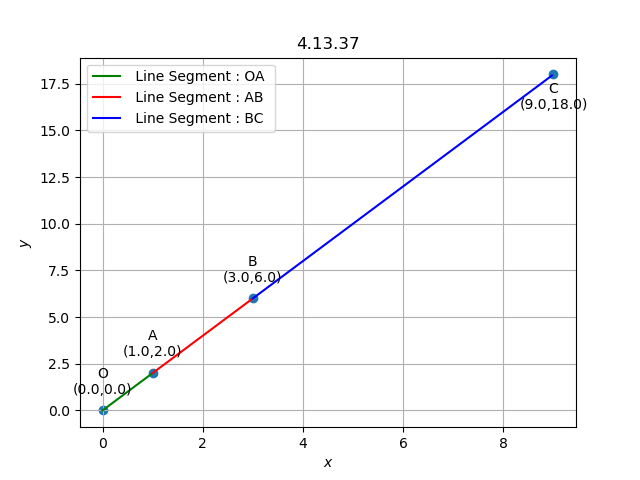
\includegraphics[width=1.0\columnwidth]{figs/colli1.png}
    \caption*{}
    \label{fig:}
\end{figure}

\end{document}

